\documentclass[11pt]{../../TexTemplate/elegantbook} % 这里是文档类,默认使用 elegantbook

\title{Géométrie Analytique} % 这里放置书名
% \subtitle{Subtitle} % 这里放置副标题

\author{CatMono} % 这里放置作者名
\date{October, 2025} % 这里放置日期
\version{0.1} % 这里放置版本号
% \institute{Elegant\LaTeX{} Program} % 这里放置机构名
% \bioinfo{Custom Key}{Custom Value} % 这里放置自定义信息

% \extrainfo{extra information} % 这里放置额外信息,将显示在最下方中央

\setcounter{tocdepth}{2} % 设置目录深度
\setcounter{secnumdepth}{2} % 设置章节编号深度


% \logo{logo-blue.png} % 这里放置封面logo,默认从figure目录下寻找
% \cover{LogiqueMathematique.png} % 这里放置封面图片,默认从figure目录下寻找

% modify the color in the middle of titlepage
\definecolor{customcolor}{RGB}{32,178,170} % 自定义颜色
\colorlet{coverlinecolor}{customcolor}
\usepackage{cprotect} % 保护命令参数不被 LaTeX 解析器过早处理,允许在某些特殊环境中使用脆弱命令(fragile commands)。
\usepackage{xeCJK} % 使用 xeCJK 包支持中文


% ===== 开始文档 =====
\begin{document}

\maketitle %生成文档的标题页,根据之前定义的标题信息(如标题、作者、日期等)自动创建一个格式化的标题页

% === 前言部分 ===
\frontmatter        % 开始前言,页码为 i, ii, iii...
\tableofcontents    % 目录 (页码: i, ii)
% \listoffigures      % 图表目录 (页码: iii)
% \listoftables       % 表格目录 (页码: iv)

\chapter{Preface}   % 前言章节(无编号,页码: v, vi...)
This is the preface of the book...

% \chapter{Acknowledgments}  % 致谢(无编号)
% I would like to thank...
% === 正文部分 ===
\mainmatter         % 开始正文,页码从 1 重新开始

\chapter{Preliminaries} % 这里放置章节标题

\chapter{Coordinates and Vectors}
\section{Coordinate Systems}
\begin{definition}{Coordinate Frame}
    A fixed point \(O\) in \(\mathbb{R}^{3}\) space,
    together with three non-coplanar ordered vectors \(\mathbf{e}_{1}, \mathbf{e}_{2}, \mathbf{e}_{3}\),
    is called a \textbf{coordinate frame} (or \textbf{reference frame}) in space,
    denoted by \(\{O ; \mathbf{e}_{1}, \mathbf{e}_{2}, \mathbf{e}_{3}\}\).

    If \(\mathbf{e}_{1}, \mathbf{e}_{2}, \mathbf{e}_{3}\) are unit vectors,
    then the frame is called a \textbf{Cartesian frame}.
    Furthermore, if \(\mathbf{e}_{1} \perp \mathbf{e}_{2}, \mathbf{e}_{2} \perp \mathbf{e}_{3}, \mathbf{e}_{3} \perp \mathbf{e}_{1}\),
    then the frame is called a \textbf{rectangular Cartesian frame}, or simply a \textbf{rectangular frame}.

    Generally, \(\{O ; \mathbf{e}_{1}, \mathbf{e}_{2}, \mathbf{e}_{3}\}\) is called \textbf{affine frame}.
\end{definition}

\section{Theorems about Vectors}

\section{Products of Vectors}
\begin{leftbarTitle}{Inner Product (Dot Product)}\end{leftbarTitle}

\begin{leftbarTitle}{Outer Product (Cross Product)}\end{leftbarTitle}

\begin{leftbarTitle}{Mixed Product}\end{leftbarTitle}

\begin{leftbarTitle}{Double Cross Product}\end{leftbarTitle}

\section{Linear Independence}

\chapter{Locus and Equation}
\section{Parametric Equations}

\section{Common Curves and Surfaces}

\chapter{Planes and Space Lines}
\section{Equations of Planes}
\begin{leftbarTitle}{Point-Vector Form}\end{leftbarTitle}
In space, fix a point \(M_{0} = (X_{0}, Y_{0}, Z_{0})\) and two non-collinear vectors \(\mathbf{a} = (X_{1}, Y_{1}, Z_{1})\) 
and \(\mathbf{b} = (X_{2}, Y_{2}, Z_{2})\).
The equation of the plane passing through the point \(M_{0}\) and 
parallel to the vectors \(\mathbf{a}\) and \(\mathbf{b}\) is given by:
\[
\mathbf{r} = \vec{OM} + \lambda \mathbf{a} + \mu \mathbf{b},
\]
or in coordinate form:
\[
\begin{cases}
x = X_{0} + \lambda X_{1} + \mu X_{2} \\
y = Y_{0} + \lambda Y_{1} + \mu Y_{2} \\
z = Z_{0} + \lambda Z_{1} + \mu Z_{2}
\end{cases}
\]
where \(\lambda, \mu \in \mathbb{R}\).

Taking the dot product of both sides of the parametric vector equation with \(\mathbf{a} \times \mathbf{b}\), 
we eliminate \(\lambda\) and \(\mu\) to obtain \((\mathbf{r} - \vec{OM_{0}}, \mathbf{a}, \mathbf{b}) = 0\), that is,
\begin{equation}\label{eq:PlaneDeterminantForm}
    \begin{vmatrix}
        x - X_{0} & y - Y_{0} & z - Z_{0} \\
        X_{1} & Y_{1} & Z_{1} \\
        X_{2} & Y_{2} & Z_{2}
    \end{vmatrix} = 0.
\end{equation}
All above forms are called the \textbf{point-vector form} of the plane equation.
\vspace{0.7cm}

Given three non-collinear points \(M_{1}(X_{1}, Y_{1}, Z_{1})\), \(M_{2}(X_{2}, Y_{2}, Z_{2})\) and \(M_{3}(X_{3}, Y_{3}, Z_{3})\),
the equation of the plane passing through these three points is given by:
\[
\mathbf{r} = \vec{OM_{1}} + \lambda \vec{M_{1}M_{2}} + \mu \vec{M_{1}M_{3}},
\]
or in coordinate form:
\[
\begin{cases}
x = X_{1} + \lambda (X_{2} - X_{1}) + \mu (X_{3} - X_{1}) \\
y = Y_{1} + \lambda (Y_{2} - Y_{1}) + \mu (Y_{3} - Y_{1}) \\
z = Z_{1} + \lambda (Z_{2} - Z_{1}) + \mu (Z_{3} - Z_{1})
\end{cases}
\]
where \(\lambda, \mu \in \mathbb{R}\).
And the determinant form is:
\[
\begin{vmatrix}
x - X_{1} & y - Y_{1} & z - Z_{1} \\
X_{2} - X_{1} & Y_{2} - Y_{1} & Z_{2} - Z_{1} \\
X_{3} - X_{1} & Y_{3} - Y_{1} & Z_{3} - Z_{1}
\end{vmatrix} = 0,
\]
or equivalently,
\[
\begin{vmatrix}
x & y & z & 1 \\
X_{1} & Y_{1} & Z_{1} & 1 \\
X_{2} & Y_{2} & Z_{2} & 1 \\
X_{3} & Y_{3} & Z_{3} & 1
\end{vmatrix} = 0.
\]
All above forms are also called the \textbf{three-point form} of the plane equation.

If plane intersects the three coordinate axes at 
\(M_{1}(X_{1}, 0, 0)\), \(M_{2}(0, Y_{2}, 0)\), \(M_{3}(0, 0, Z_{3})\) (where \(X_{1}, Y_{2}, Z_{3} \neq 0\)), 
then the equation of the plane can be expressed in the form:
\[
\frac{x}{X_{1}} + \frac{y}{Y_{2}} + \frac{z}{Z_{3}} = 1,
\]
which is called the \textbf{intercept form} of the plane equation.

\begin{leftbarTitle}{General Form}\end{leftbarTitle}
The general equation is obtained by expanding the determinant form of 
the parametric equation~\ref{eq:PlaneDeterminantForm} of a plane:
\[
Ax + By + Cz + D = 0,
\]
where
\[
A = \begin{vmatrix} Y_{1} & Z_{1} \\ Y_{2} & Z_{2} \end{vmatrix}, \quad
B = \begin{vmatrix} Z_{1} & X_{1} \\ Z_{2} & X_{2} \end{vmatrix}, \quad
C = \begin{vmatrix} X_{1} & Y_{1} \\ X_{2} & Y_{2} \end{vmatrix}, \quad
D = -\begin{vmatrix} X_{0} & Y_{0} & Z_{0} \\ X_{1} & Y_{1} & Z_{1} \\ X_{2} & Y_{2} & Z_{2} \end{vmatrix}.
\]
Special cases include:

\begin{theorem}
    Any plane in space can be represented by a linear equation in three variables \(x\), \(y\), and \(z\), 
    and conversely, every such equation represents a plane in space.
\end{theorem}

\begin{leftbarTitle}{Point-Normal Form}\end{leftbarTitle}

\section{Linear Equations}

\section{Relative Positions of Points, Lines and Planes}

\section{Pencil of Planes and Lines}

\chapter{Common Surfaces}
\section{Cylinder Surfaces}

\section{Cone Surfaces}

\section{Surfaces of Revolution}

\section{Quadric Surfaces}

\chapter{Conic Sections}
\section{General Equation of Conic Sections}

\begin{figure}[h]
    \centering
    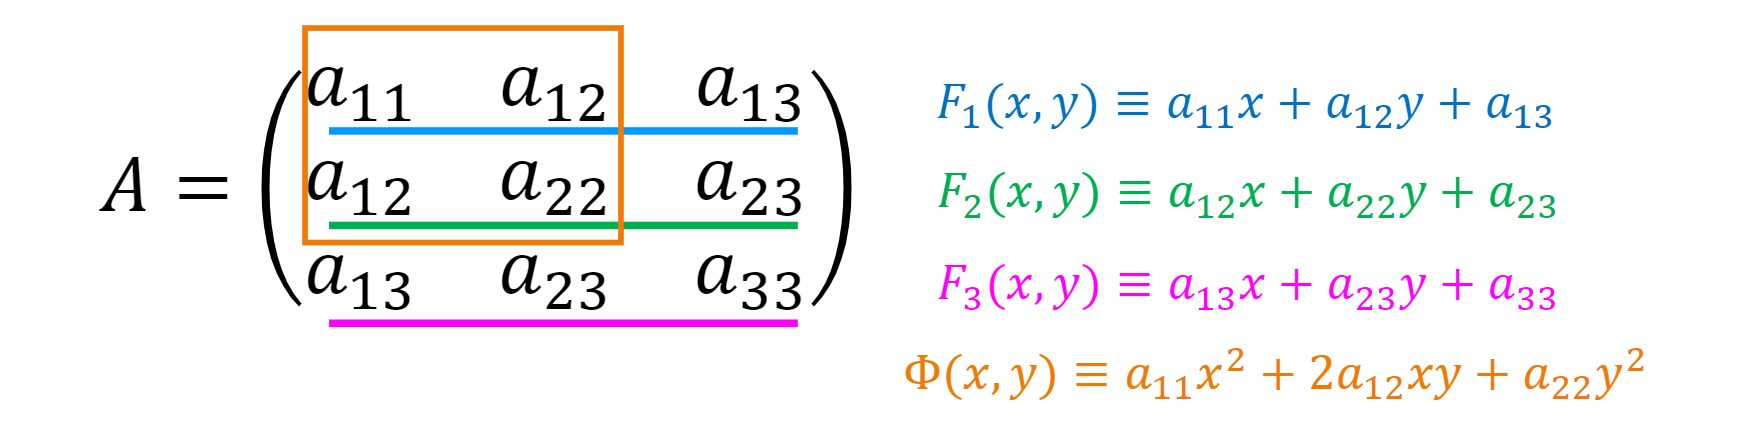
\includegraphics[width=0.8\textwidth]{img/ConicRelation.png}
\end{figure}

\section{Conic Sections and Lines}

\section{Simplification of Conic Equations}




\begin{thebibliography}{99} 
\bibitem{en1} 作者, Title1, Journal1, Year1. \emph{ This is an example of a reference.}
\bibitem{en2} Author2, Title2, Journal2, Year2. \emph{ This is another example of a reference.}
\end{thebibliography}

\end{document}